\chapter{Grundlagen}

Folgend werden die wissenschaftlichen Grundlagen dargelegt, auf denen die in dieser Arbeit eingesetzten Konzepte beruhen. Zum Verstehen dieser Arbeit ist ein grundlegendes Verständnis von Physik und Akustik vorauszusetzen \cite{Lerch2009, Mueller2004}. Weiteres Fachwissen sowie die zum Verstehen dieser Arbeit notwendigen Grundlagen werden in diesem Kapitel erläutert. 


\section{DML-Technologie}

Die Abkürzung DML steht für Distributed Mode Loudspeaker, dabei handelt es sich um einen Lautsprecher, welcher sich von konventionellen Membranlautsprechern grundlegend unterscheidet. Ein DML, auch bekannt als Flach- oder Panel-Lautsprecher, ist eine Bauform eines Biegewellenwandlers, bei der eine Platte oder ein Panel mithilfe eines elektrodynamischen Körperschallwandlers, welcher auch als Exciter bezeichnet wird, angeregt wird. Bei dieser Anregung entstehen Plattenbiegewellen, die auf der Oberfläche der Platte verlaufen. Die Schwingungen werden von der Gesamtoberfläche abgestrahlt und erzeugen somit hörbaren Schall \cite{Moeser2005, Li2010, TectonicAudioLabs2013}. Damit stellen DML-Flachlautsprecher eine Alternative zur konventionellen Kolbenstrahler-Technologie dar. Denn im Gegensatz zu klassischen Lautsprechern, wo die Lautsprechermembran angeregt kolbenartige Bewegungen ausführt, basiert die DML-Technologie auf der gezielten Anregung von Biegewellen in einer Platte. 
Bei einem DML-Flachlautsprecher breiten sich die vom Exciter erzeugten Anregungen konzentrisch vom Anregungspunkt aus, wie Wellen auf einer Wasseroberfläche. Die Biegewellengeschwindigkeit ist dabei nicht konstant, sondern frequenzabhängig, da Biegewellen dispersiv sind \cite{Moeser2005}. Dies bedeutet, dass höhere Frequenzen sich schneller auf der Platte ausbreiten als niedrige \cite{Redondo2007}. Im Gegensatz zu Longitudinalwellen in Gasen, die eine konstante Ausbreitungsgeschwindigkeit besitzen \cite{DEGA2006}, erzeugt diese Dispersion auf dem DML-Panel eine frequenzabhängige Interferenz verschiedener Moden, die wiederum das charakteristische Abstrahlmuster von DML-Flachlautsprechern bestimmt.


Ein zentrales Merkmal eines DML-Flachlautsprechers ist die sogenannte Koinzidenzfrequenz. Bei dieser Frequenz stimmt die Biegewellengeschwindigkeit auf der Platte mit der Schallgeschwindigkeit in der umgebenden Luft überein. Unterhalb der Koinzidenzfrequenz strahlt die Platte diffus und omnidirektional ab, die Schallabstrahlung erfolgt nicht aus einer kohärenten Wellenfläche, sondern durch die Überlagerung zahlreicher, zum Teil gegenphasiger Flächenelemente \cite{Cremer1996}. Oberhalb der Koinzidenzfrequenz hingegen wird die Abstrahlung deutlich effizienter, da sich die Biegewellen auf der Platte phasenkohärent mit der umgebenden Luftschallwelle koppeln können. Diese beiden Betriebsbereiche prägen das Gesamtverhalten von DML-Flachlautsprechern.

\begin{figure}[H]
	\centering
	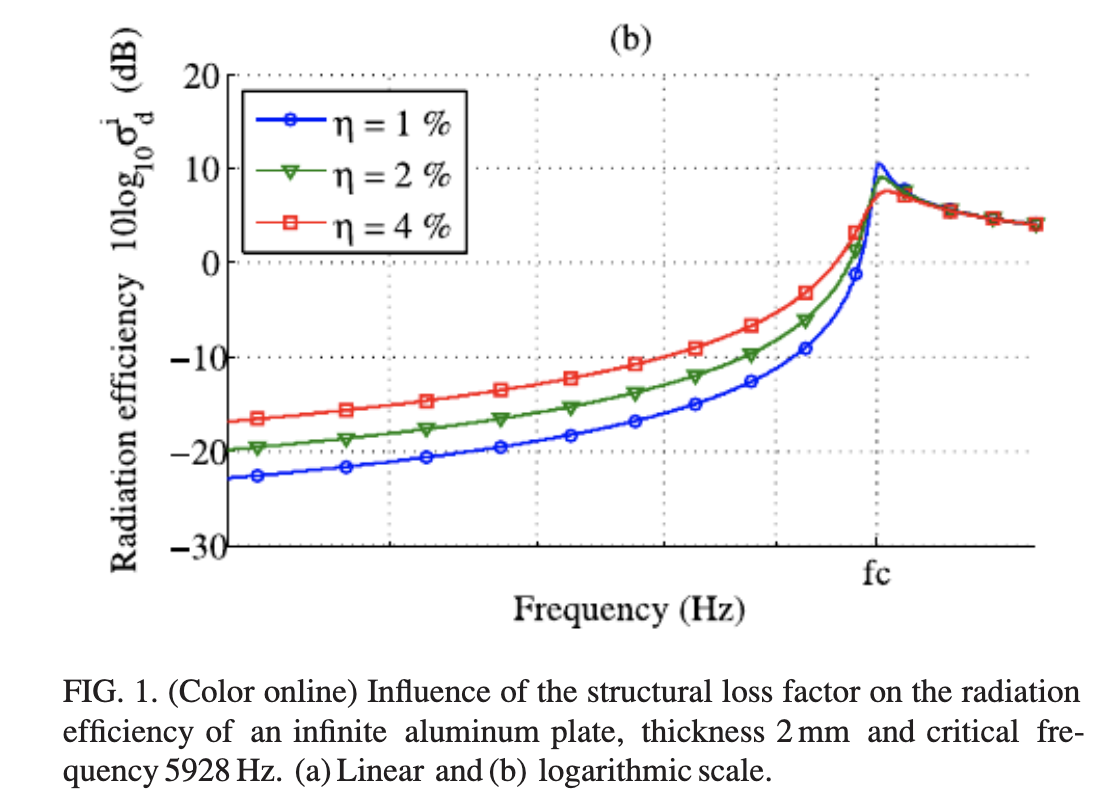
\includegraphics[width=0.9\textwidth]{pictures/Koinzidenzfrequenz.png}
	\caption[Abstrahlgrad einer gedämpften Platte in Abhängigkeit von der Frequenz]{Abstrahlgrad einer gedämpften, unendlich ausgedehnten Aluminiumplatte mit Dicke \SI{2}{\milli\meter} und kritischer Frequenz $f_c = \SI{5928}{\hertz}$ in Abhängigkeit von der Frequenz für die Verlustfaktoren $\eta = 1\,\%$, $2\,\%$ und $4\,\%$ in logarithmischer Darstellung \cite{Kou2015}.}
	\label{fig:koinzidenzfrequenz}
\end{figure}

Abbildung~\ref{fig:koinzidenzfrequenz} zeigt den Abstrahlgrad $\sigma$ einer Platte in Abhängigkeit von der Frequenz für drei Verlustfaktoren $\eta$ nach Kou et al.\ \cite{Kou2015}. Im unterkritischen Bereich mit $f < f_c$ liegt die Biegewellengeschwindigkeit unter der Schallgeschwindigkeit der Luft, wodurch ein akustischer Kurzschluss entsteht und $\sigma$ deutlich unter 1 bleibt \cite{Cremer1996}. In diesem Bereich beeinflusst die Materialdämpfung den Abstrahlgrad merklich. Mit zunehmendem Verlustfaktor steigt der Abstrahlgrad, da die Dämpfung die Modenamplituden begrenzt und so die Phasenkohärenz zur umgebenden Luft verbessert \cite{Kou2015}. Bei der Koinzidenzfrequenz $f \approx f_c$ ist die Spuranpassungsbedingung erfüllt und $\sigma$ erreicht ein Maximum. Im überkritischen Bereich mit $f > f_c$ nähert sich $\sigma$ asymptotisch dem Wert 1 bei zunehmend gerichteter Abstrahlung \cite{Moeser2010}.

Beim DML-Lautsprecher wird durch gezielte Exciter-Positionierung und geeignetes Seitenverhältnis die Modendichte so erhöht, dass der Koinzidenz-Peak zu einem breiten Plateau mit $\sigma \approx 0{,}5$--$1$ verschmiert -- dies entspricht der Designabsicht diffuser DML-Abstrahlung \cite{Beer1999}.


Der Vorteil eines DML-Flachlautsprechers liegt vor allem in seinem breiten, räumlich gleichmäßigen Schallfeld, das sich durch die diffuse Abstrahlung in einem weiten Frequenzbereich ergibt. Dies macht diese Lautsprecherbauform besonders attraktiv für Anwendungen, bei denen eine homogene Beschallung eines Raumes ohne starke Schallbündelung gefordert ist \cite{Beer1999, KuhnRahloff2025}. Gleichzeitig sind der verhältnismäßig niedrige Wirkungsgrad im Tieffrequenzbereich sowie die irregulären Resonanzspitzen im Frequenzgang typische Nachteile. 

\subsection{Material-Parameter und deren Einfluss}

Die Materialeigenschaften des angeregten Panels prägen die resultierende Abstrahlcharakteristik und damit das akustische Verhalten maßgeblich. Die für die Akustik wichtigsten Eigenschaften eines DML-Panels werden durch zwei Parameter bestimmt, die Biegesteifigkeit $B$ und die Flächenmasse $m''$. Beide Größen stehen in direkter Beziehung zu den Eigenfrequenzen der Platte. Nach der Kirchhoff-Plattentheorie lassen sich die Eigenfrequenzen der $(m,n)$-ten Mode einer rechteckigen Platte mit den Seitenlängen $a$ und $b$ gemäß Gleichung~\ref{eq:eigenfrequenz} berechnen \cite{Cremer1996}.

\begin{equation}
f_{m,n} = \frac{\pi}{2} \sqrt{\frac{B}{m''}} \left( \left(\frac{m}{a}\right)^2 + \left(\frac{n}{b}\right)^2 \right)
\label{eq:eigenfrequenz}
\end{equation}

\begin{itemize}
    \item $f_{m,n}$ : Eigenfrequenz der $(m,n)$-ten Mode $[\text{Hz}]$
    \item $B$ : Biegesteifigkeit $[\text{Nmm}^2]$
    \item $m''$ : Flächenmasse $[\text{kg/m}^2]$
    \item $a$, $b$ : Seitenlängen der Platte $[\text{m}]$
    \item $m$, $n$ : Modenindizes
\end{itemize}

Aus Gleichung~\ref{eq:eigenfrequenz} folgt, dass eine höhere Biegesteifigkeit $B$ die Eigenfrequenzen anhebt, während eine größere Flächenmasse $m''$ sie absenkt \cite{Cremer1996}. Für ein ausgewogenes akustisches Verhalten ist daher ein abgestimmtes Verhältnis von Biegesteifigkeit und Flächenmasse erforderlich. Eine zu hohe Biegesteifigkeit verschiebt die Eigenfrequenzen zu höheren Werten und erschwert die Anregung im Tieffrequenzbereich. Eine zu geringe Biegesteifigkeit erzeugt dagegen eine hohe modale Dichte bei niedrigen Frequenzen, was eine verlängerte Ausschwingzeit zur Folge hat.

Eine hohe Biegesteifigkeit bei gleichzeitig geringer Flächenmasse wird durch Sandwichkonstruktionen erreicht, die sich daher als geeignete DML-Panele etabliert haben \cite{Bai2001}. Der Aufbau besteht aus zwei dünnen, biegesteifen Deckschichten, die durch einen leichten Stützkern auf Abstand gehalten werden. Die Deckschichten tragen den überwiegenden Anteil der Biegebelastung, während der Kern die Schubsteifigkeit liefert und die Deckschichten gegen Beulen stützt \cite{Wiedemann2006}. Die effektive Biegesteifigkeit einer solchen Konstruktion lässt sich näherungsweise mit Gleichung~\ref{eq:biegesteifigkeit} berechnen.

\begin{equation}
B \approx E \cdot T \cdot \left(\frac{d-T}{2}\right)^2
\label{eq:biegesteifigkeit}
\end{equation}

\begin{itemize}
    \item $B$ : Biegesteifigkeit $[\text{Nmm}^2]$
    \item $E$ : Elastizitätsmodul $[\text{N/mm}^2]$
    \item $T$ : Stärke der Deckschicht $[\text{mm}]$
    \item $d$ : Gesamtstärke der Platte $[\text{mm}]$
\end{itemize}

Der quadratische Zusammenhang zeigt, dass bereits eine geringe Erhöhung der Gesamtdicke $d$ eine erhebliche Steigerung der Biegesteifigkeit bewirkt \cite{Wiedemann2006}. Im Vergleich zu monolithischen Platten erreichen Sandwichkonstruktionen bei gleicher Biegesteifigkeit eine deutlich geringere Flächenmasse, was die modale Dichte und damit den Frequenzgang vorteilhaft beeinflusst.

Neben Steifigkeit und Masse spielt die innere Dämpfung des Panelmaterials eine wesentliche Rolle. Eine zu geringe Dämpfung führt zu langanhaltenden Resonanzspitzen im Frequenzgang und damit zu hörbaren Klangverfärbungen. Eine zu hohe Dämpfung reduziert dagegen die Schallabstrahlungseffizienz und kann das transiente Verhalten der Platte verschleiern \cite{Moeser2010}. Ein abgestimmtes Dämpfungsniveau hält die Resonanzamplituden in Grenzen, ohne die Abstrahlung wesentlich zu beeinträchtigen. Bei der Materialauswahl ist daher das Verhältnis von Steifigkeit, Masse und Dämpfung gemeinsam zu betrachten. Ein niedriges Verhältnis $B/m''$ erhöht die Modendichte und senkt die erste Eigenfrequenz \cite{Moeser2010}; gleichzeitig muss eine ausreichende innere Dämpfung vorhanden sein, um Resonanzspitzen zu unterdrücken.

Tabelle~\ref{tab:materialvergleich} stellt verschiedene Materialien anhand ihrer Flächenmasse $m''$ und ihrer inneren Dämpfung gegenüber. Die Dämpfung ist dabei in die Kategorien \glqq sehr niedrig\grqq{} bis \glqq mittel\grqq{} gegliedert.

\begin{table}[htbp]
\centering
\caption{Materialvergleich für DML}
\label{tab:materialvergleich}
\footnotesize
\setlength{\tabcolsep}{3pt}
\begin{tabularx}{\textwidth}{|p{2.5cm}|p{2.5cm}|c|c|c|X|}
\hline
\textbf{Material} & \textbf{Struktur} & \textbf{m''} & \textbf{Dämpfung} & \textbf{Eignung} & \textbf{Begründung} \\
 & & \textbf{[g/m²]} & & & \\
\hline
CFK/Nomex-Honeycomb & Sandwich: CFK + Nomex-Kern & 35--80 & mittel & $\checkmark\checkmark$ &
\vspace{-2mm}
\begin{itemize}[leftmargin=*, nosep, topsep=0pt, parsep=0pt]
    \item Höchste B/m''-Klasse
    \item Niedrige Masse
    \item Ideal für prof. DML
\end{itemize}
\vspace{-2mm} \\
\hline
Balsa/CFK-Sandwich & Sandwich: CFK + Balsa-Kern & 80--150 & mittel--niedrig & $\checkmark\checkmark$ &
\vspace{-2mm}
\begin{itemize}[leftmargin=*, nosep, topsep=0pt, parsep=0pt]
    \item Sehr hohe spez. Biegesteifigkeit
    \item Gut für Niederfrequenz-DML
\end{itemize}
\vspace{-2mm} \\
\hline
XPS (20\,mm) & Monolithisch & 160--200 & mittel & $\checkmark$ &
\vspace{-2mm}
\begin{itemize}[leftmargin=*, nosep, topsep=0pt, parsep=0pt]
    \item DIY-Material
    \item Gute Dämpfung
    \item Für Höchstfrequenzen
\end{itemize}
\vspace{-2mm} \\
\hline
KAPA\textsuperscript{\textregistered}line 15\,mm\textsuperscript{*} & Sandwich: PU + Karton & 1.037 & mittel & $\circ$ &
\vspace{-2mm}
\begin{itemize}[leftmargin=*, nosep, topsep=0pt, parsep=0pt]
    \item m'' zu hoch
    \item Als Prototyp möglich
\end{itemize}
\vspace{-2mm} \\
\hline
KAPA\textsuperscript{\textregistered}graph 5\,mm\textsuperscript{*} & Sandwich: PU + Karton & 715 & mittel & $\circ$ &
\vspace{-2mm}
\begin{itemize}[leftmargin=*, nosep, topsep=0pt, parsep=0pt]
    \item Leichter als KAPA\textsuperscript{\textregistered}line
    \item Steifere Deckschichten
\end{itemize}
\vspace{-2mm} \\
\hline
Sperrholz (4\,mm) & monolithisch (Leimholz) & 1.200--1.600 & niedrig & $\circ$ &
\vspace{-2mm}
\begin{itemize}[leftmargin=*, nosep, topsep=0pt, parsep=0pt]
    \item Anisotrop
    \item Masse zu hoch
\end{itemize}
\vspace{-2mm} \\
\hline
Gipskarton & monolithisch & 8.000--12.000 & sehr niedrig & $\times$ &
\vspace{-2mm}
\begin{itemize}[leftmargin=*, nosep, topsep=0pt, parsep=0pt]
    \item Sehr hohe Masse
    \item Keine Abstrahlung möglich
\end{itemize}
\vspace{-2mm} \\
\hline
Aluminium (1\,mm) & monolithisch & 2.700 & sehr niedrig & $\times$ &
\vspace{-2mm}
\begin{itemize}[leftmargin=*, nosep, topsep=0pt, parsep=0pt]
    \item Masse zu groß
    \item Dämpfung $\approx$ 0
    \item Resonanzspitzen
\end{itemize}
\vspace{-2mm} \\
\hline
\end{tabularx}

\vspace{0.2cm}
\scriptsize
\textbf{Legende:} $\checkmark\checkmark$ sehr geeignet \quad $\checkmark$ geeignet \quad $\circ$ bedingt geeignet \quad $\times$ nicht geeignet \quad
\textsuperscript{*} Datenblatt 3A Composites, 06/2021

\textbf{Quellen:} \cite{Moeser2005}; \cite{Zenker2019}; 3A Composites GmbH; \cite{Wiedemann2006}; \cite{EngineeringRadio2021}.
\end{table}

Die Tabelle führt in den ersten beiden Spalten den Materialnamen und den strukturellen Aufbau auf, gefolgt von Flächenmasse und Dämpfungsklasse. Die fünfte Spalte bewertet die Eignung als DML-Material anhand der in der Legende erläuterten Symbole; die sechste Spalte ergänzt diese Einschätzung um eine kurze Begründung. Die Materialien sind nach absteigender Eignung sortiert.


\subsection{Exciter-Position und deren Einfluss}

Die Position des Körperschallwandlers auf dem DML-Panel hat einen entscheidenden Einfluss darauf, welche Eigenmoden im Panel angeregt werden und wie effizient diese zur Schallabstrahlung beitragen. Jede Mode in einem endlichen Panel besitzt charakteristische Eigenformen und Knotenpunkte, an diesen Stellen geht die Schwingungsamplitude gegen null. Wenn ein Körperschallwandler auf einem Knotenpunkt platziert wird, kann die entsprechende Mode nicht wirksam angeregt werden. Die Platzierung des Körperschallwandlers ist daher von zentraler Bedeutung, um eine gleichmäßige Modenanregung über den Frequenzbereich zu erhalten. 

Eine symmetrische Anordnung des Exciters in der Panelmitte ist aus physikalischer Sicht unvorteilhaft, da in der Mitte eines rechteckigen Panels zahlreiche Knotenpunkte indizierter Moden zusammenfallen. Somit können von diesem Exciter nicht alle Moden angeregt werden \cite{Moeser2010}. Aus diesem Grund wird sowohl von Exciter-Herstellern als auch in der Fachliteratur eine asymmetrische Positionierung des Exciters empfohlen \cite{Bai2001, DaytonAudio2024}.

Eine Studie der Technischen Universität Dresden analysierte die Positionierung von Excitern auf einem rechteckigen DML-Panel anhand von fünfundzwanzig unterschiedlichen Anregungspunkten mittels numerischer Simulation. Die dabei erzielten Ergebnisse zeigen, dass die optimale Anreger-Position maßgeblich von der Panelgeometrie und deren Maßen, den Materialeigenschaften sowie vom gewünschten Frequenzbereich abhängt. Die Analyse erfolgte auf Basis der in der Simulation berechneten abgestrahlten Schallleistung. Eine universell optimale Exciter-Position, welche von der Panelgeometrie und deren Materialeigenschaften unabhängig ist, konnte im Rahmen der Untersuchung ausgeschlossen werden. \cite{Zenker2019}

 
\section{Vergleich DML zu konventionellen Lautsprechern}

Konventionelle Lautsprecher basieren auf dem Prinzip der Kolbenbewegung, bei der eine Membran, welche meist konisch geformt ist, durch eine Schwingspule in Bewegung versetzt wird. Diese Vor- und Rückbewegung verdrängt Luft und erzeugt Schallwellen \cite{Harris2000, Bernstein2019}.
Der DML-Flachlautsprecher, wie in Kapitel 2.1 beschrieben, erzeugt durch die Anregung eines Exciters sich überlagernde Biegewellen, welche sich auf einem Panel ausbreiten und dadurch Schallwellen erzeugen. 

\begin{figure}[H]
	\centering
	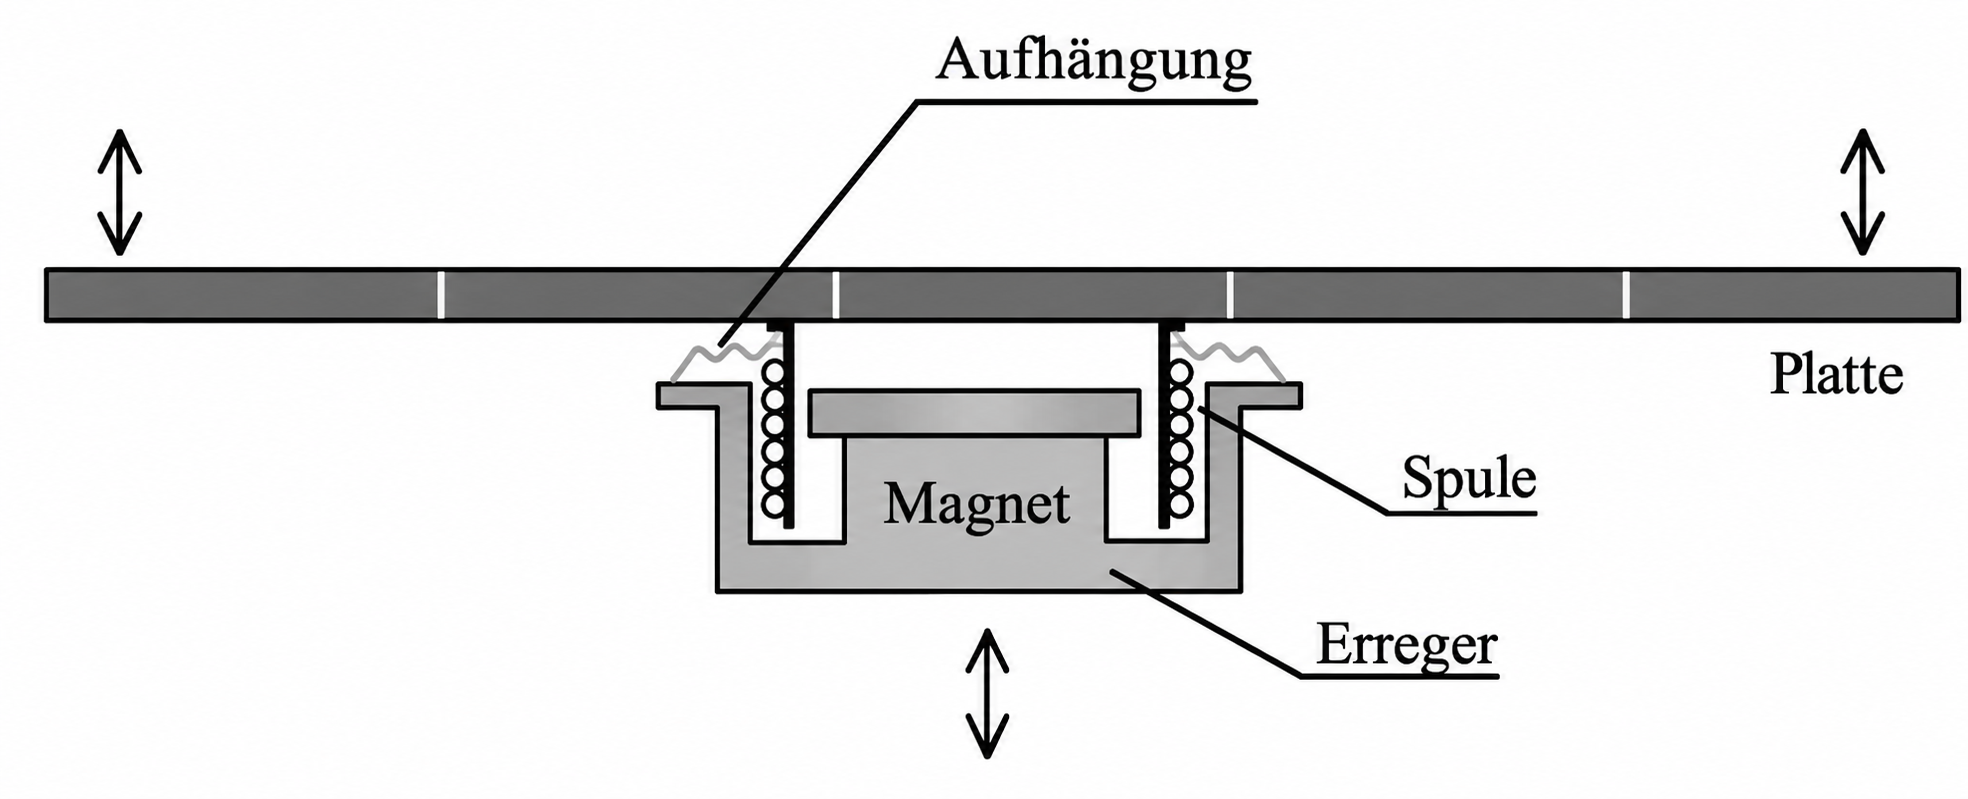
\includegraphics[width=0.8\textwidth]{pictures/DML_aufbau.png}
	\caption{Aufbau eines DML-Lautsprechers \cite{Bai2001}}
	\label{fig:DML_aufbau}
\end{figure}

In Abbildung \ref{fig:DML_aufbau} ist der Aufbau eines DML-Lautsprechers abgebildet. Dabei ist unten im Bild der Exciter zu erkennen, welcher aus einem Magneten sowie einer Spule besteht. Beim Aufbau des elektromagnetischen Anregungsmechanismus unterscheidet sich der DML nur wenig zum konventionellen Lautsprecher. Durch das Ansteuern des Exciters wird die Klebefläche, welche mit dem Panel verklebt ist, in Schwingung versetzt. Diese Schwingung wird auf das Panel übertragen. 


\begin{figure}[H]
	\centering
	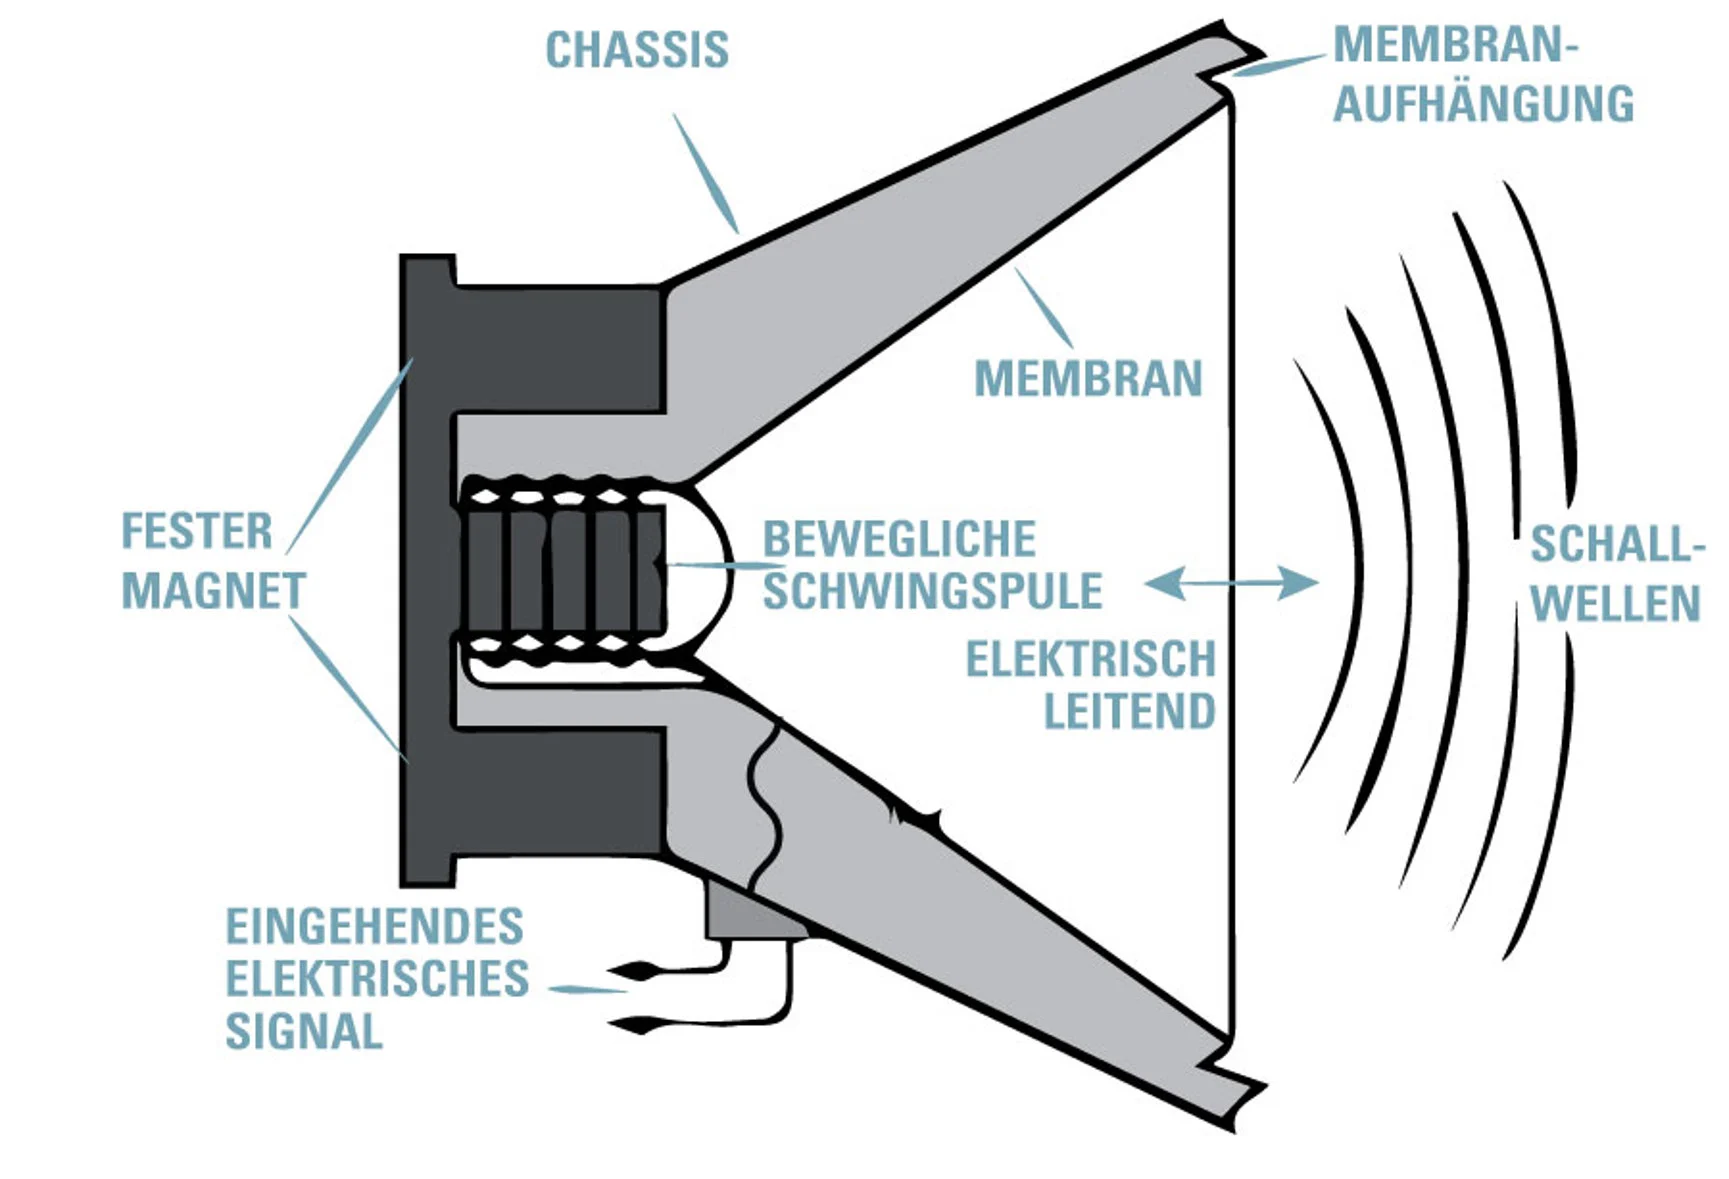
\includegraphics[width=0.8\textwidth]{pictures/Lautsprecher_aufbau.png}
	\caption{Aufbau eines konventionellen Lautsprechers \cite{HiFiKlubben}}
	\label{fig:Lautsprecher_aufbau}
\end{figure}

Abbildung \ref{fig:Lautsprecher_aufbau} zeigt den Aufbau eines konventionellen Membranlautsprechers. Zu erkennen ist, dass die Membran mit der Spule verbunden ist und diese bei Anregung in Schwingung versetzt wird.

\begin{figure}[H]
	\centering
	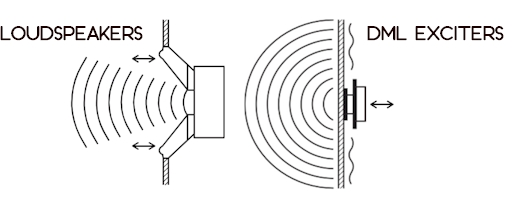
\includegraphics[width=0.8\textwidth]{pictures/Abstrahl Charakteristik.jpg}
	\caption{Abstrahlverhalten eines DML-Lautsprechers im Vergleich zu einem konventionellen Lautsprecher \cite{JGJMatt2023, ExcitersCN}}
	\label{fig:Abstrahlverhalten}
\end{figure}

Abbildung \ref{fig:Abstrahlverhalten} zeigt das unterschiedliche Abstrahlverhalten eines DML-Lautsprechers im Vergleich zu einem konventionellen Lautsprecher. Während der konventionelle Lautsprecher mit zunehmender Frequenz eine stärkere Bündelung aufweist, behält der DML-Lautsprecher eine breitere, nahezu omnidirektionale Abstrahlung über einen weiten Frequenzbereich bei.

Ein bedeutender Vorteil von DML-Lautsprechern liegt in ihrer flachen, leichten und konstruktiv gut integrierbaren Bauweise, was im Vergleich der Abbildungen \ref{fig:DML_aufbau} und \ref{fig:Lautsprecher_aufbau} gut zu erkennen ist. Da das abstrahlende Element selbst eine Platte ist, lassen sich DML-Systeme vergleichsweise unauffällig in Fahrzeuginnenräumen, Möbeln, Displays oder Wandstrukturen integrieren. Insbesondere in Anwendungen mit begrenztem Bauraum oder hohen Anforderungen an Design und Flächenintegration bieten sie daher konstruktive Vorteile gegenüber klassischen Lautsprechern mit Korb, Magnetantrieb und definierter Membrangeometrie.

Akustisch zeigen die beiden Systeme jedoch unterschiedliche Stärken und Schwächen. Konventionelle Lautsprecher erreichen in der Regel eine bessere Kontrolle des Tieftonbereichs, einen höheren Wirkungsgrad in dafür optimierten Gehäusekonzepten sowie eine insgesamt besser vorhersagbare Abstimmung des Frequenzgangs.
DML-Systeme weisen demgegenüber konstruktionsbedingt häufig Defizite im Bassbereich auf, da große Hubbewegungen und eine gezielte tieffrequente Luftverdrängung nur eingeschränkt möglich sind. Daher benötigen DML- und Multiactor-Panel-Systeme zur Verbesserung ihrer Tieftonwiedergabe häufig zusätzliche Entzerrung, spezielle Randbedingungen oder ergänzende konstruktive Maßnahmen.

Auch hinsichtlich der Richtcharakteristik bestehen deutliche Unterschiede. Konventionelle Lautsprecher zeigen typischerweise eine mit steigender Frequenz zunehmende Bündelung, sofern keine besonderen Maßnahmen zur Direktivitätskontrolle getroffen werden. DML-Lautsprecher werden dagegen häufig mit einer breiten und teilweise quasi-omnidirektionalen Abstrahlung im Mittel- und Hochtonbereich in Verbindung gebracht. Diese Eigenschaft kann vorteilhaft sein, wenn eine räumlich diffuse und umhüllende Wiedergabe erwünscht ist. Gleichzeitig kann gerade diese breite Abstrahlung aber auch nachteilig sein, da sie zu einer geringeren Lokalisationsschärfe und zu stärkerer raumabhängiger Wiedergabe sowie zu einer weniger konstanten Off-Axis-Charakteristik führen kann.

Aus systemtechnischer Sicht ist außerdem zu berücksichtigen, dass DML-Lautsprecher häufig eine aufwendigere Abstimmung benötigen. Die vibroakustischen Eigenschaften hängen nicht nur stark von Materialparametern, Plattengeometrie und Randlagerung ab sondern auch von Position und Anzahl der Exciter sowie von zusätzlichen Entzerrungsmaßnahmen. Daher ist die Entwicklung leistungsfähiger DML-Systeme in besonderem Maße von numerischer Simulation, experimenteller Modalanalyse und digitaler Signalverarbeitung geprägt.
Für konventionelle Lautsprecher existieren hingegen etablierte Auslegungs- und Ersatzmodelle, mit denen sich das Verhalten deutlich standardisierter vorhersagen lässt. Zwar können moderne DML-Systeme durch geeignete Equalization und konstruktive Optimierung deutlich verbessert werden, jedoch ist der Entwicklungsaufwand im Allgemeinen höher.


Eine eindeutige Überlegenheit eines Lautsprechersystems lässt sich hinsichtlich der subjektiven Klangwahrnehmung nicht ableiten. Entzerrte DML-Systeme können qualitativ an konventionelle Lautsprecher heranreichen und weisen insbesondere Vorteile in der räumlichen Wiedergabe, etwa hinsichtlich Umhüllung und wahrgenommener Abstrahlbreite, auf. Konventionelle Lautsprecher zeigen dagegen häufig Stärken in der Abbildungspräzision, Lokalisationsschärfe und tonalen Ausgewogenheit. Die Bewertung beider Systeme ist daher anwendungsabhängig vorzunehmen. Während DML-Systeme vor allem für flache, integrierte und designorientierte Anwendungen geeignet erscheinen, bleiben konventionelle Lautsprecher bei linearer, pegelfester und bassstarker Wiedergabe meist überlegen.

Die wesentlichen Unterschiede zwischen DML- und konventionellen Lautsprechern sind in Tabelle \ref{tab:dml_konventionell_vergleich} zusammengefasst.

\begin{table}[htbp]
\centering
\caption{Vergleich DML-Lautsprecher und konventionelle Lautsprecher}
\label{tab:dml_konventionell_vergleich}
\footnotesize
\setlength{\tabcolsep}{3pt}
\begin{tabularx}{\textwidth}{|X|X|X|}
\hline
\textbf{Eigenschaft} & \textbf{DML-Lautsprecher} & \textbf{Konventioneller Lautsprecher} \\
\hline
\textbf{Abstrahl\-charakteristik} &
\vspace{-2mm}
\begin{itemize}[leftmargin=*, nosep, topsep=0pt, parsep=0pt]
    \item Diffuse, omnidirektionale Abstrahlung unterhalb Koinzidenzfrequenz
    \item Breites Schallfeld (150--170°)
\end{itemize}
\vspace{-2mm}
&
\vspace{-2mm}
\begin{itemize}[leftmargin=*, nosep, topsep=0pt, parsep=0pt]
    \item Gerichtete Abstrahlung
    \item Frequenzabhängige Bündelung
    \item Definierter Sweet Spot
\end{itemize}
\vspace{-2mm} \\
\hline
\textbf{Tiefton\-wiedergabe} &
\vspace{-2mm}
\begin{itemize}[leftmargin=*, nosep, topsep=0pt, parsep=0pt]
    \item Eingeschränkt durch geringe Luftverdrängung
    \item Abhängig von Plattengröße und Biegesteifigkeit
    \item Subwoofer-Ergänzung oft erforderlich
\end{itemize}
\vspace{-2mm}
&
\vspace{-2mm}
\begin{itemize}[leftmargin=*, nosep, topsep=0pt, parsep=0pt]
    \item Effiziente Abstrahlung durch Kolbenbewegung
    \item Optimierbar durch Gehäusevolumen
    \item Bassreflexsysteme möglich
\end{itemize}
\vspace{-2mm} \\
\hline
\textbf{Hochton\-wiedergabe} &
\vspace{-2mm}
\begin{itemize}[leftmargin=*, nosep, topsep=0pt, parsep=0pt]
    \item Fragmentiertes Abstrahlmuster
    \item Interferenz vieler Biegemoden
    \item Starke Nebenkeulen oberhalb Koinzidenzfrequenz
\end{itemize}
\vspace{-2mm}
&
\vspace{-2mm}
\begin{itemize}[leftmargin=*, nosep, topsep=0pt, parsep=0pt]
    \item Kontrollierte Abstrahlung
    \item Separate Hochtontreiber
    \item Glatter Frequenzgang erreichbar
\end{itemize}
\vspace{-2mm} \\
\hline
\textbf{Frequenzgang} &
\vspace{-2mm}
\begin{itemize}[leftmargin=*, nosep, topsep=0pt, parsep=0pt]
    \item Unregelmäßig ($\pm$8--12\,dB)
    \item Modale Struktur
    \item Entzerrung (EQ) erforderlich
\end{itemize}
\vspace{-2mm}
&
\vspace{-2mm}
\begin{itemize}[leftmargin=*, nosep, topsep=0pt, parsep=0pt]
    \item Gleichmäßiger Verlauf
    \item Etablierte Auslegungsverfahren
    \item Geringere Schwankungen
\end{itemize}
\vspace{-2mm} \\
\hline
\textbf{Räumliche Wahrnehmung} &
\vspace{-2mm}
\begin{itemize}[leftmargin=*, nosep, topsep=0pt, parsep=0pt]
    \item Hohe räumliche Umhüllung (Envelopment)
    \item Große wahrgenommene Quellenbreite
\end{itemize}
\vspace{-2mm}
&
\vspace{-2mm}
\begin{itemize}[leftmargin=*, nosep, topsep=0pt, parsep=0pt]
    \item Präzise Lokalisation
    \item Scharfe Quellenabbildung
\end{itemize}
\vspace{-2mm} \\
\hline
\textbf{Bauform} &
\vspace{-2mm}
\begin{itemize}[leftmargin=*, nosep, topsep=0pt, parsep=0pt]
    \item Sehr flach ($<$\,20\,mm möglich)
    \item Gut integrierbar in Wände, Decken, Möbel
\end{itemize}
\vspace{-2mm}
&
\vspace{-2mm}
\begin{itemize}[leftmargin=*, nosep, topsep=0pt, parsep=0pt]
    \item Größere Bautiefe erforderlich
    \item Membran, Korb und Gehäuse
\end{itemize}
\vspace{-2mm} \\
\hline
\textbf{Wirkungsgrad} &
\vspace{-2mm}
\begin{itemize}[leftmargin=*, nosep, topsep=0pt, parsep=0pt]
    \item Niedrig im Tieftonbereich
    \item Höher bei Koinzidenzfrequenz
\end{itemize}
\vspace{-2mm}
&
\vspace{-2mm}
\begin{itemize}[leftmargin=*, nosep, topsep=0pt, parsep=0pt]
    \item Höherer Gesamtwirkungsgrad
    \item Optimierte Gehäusekonzepte
\end{itemize}
\vspace{-2mm} \\
\hline
\textbf{System\-komplexität} &
\vspace{-2mm}
\begin{itemize}[leftmargin=*, nosep, topsep=0pt, parsep=0pt]
    \item Hoch (Material, Exciter-Position, Randlagerung)
    \item FEM-Simulation oft erforderlich
\end{itemize}
\vspace{-2mm}
&
\vspace{-2mm}
\begin{itemize}[leftmargin=*, nosep, topsep=0pt, parsep=0pt]
    \item Geringer Aufwand
    \item Etablierte analytische Modelle
    \item Ersatzschaltbilder verfügbar
\end{itemize}
\vspace{-2mm} \\
\hline
\end{tabularx}

\vspace{0.2cm}
\scriptsize
\textbf{Quellen:} \cite{Harris2000}; \cite{Weinzierl2025}; \cite{Cremer1996}; \cite{Moeser2010}; \cite{Bai2001}; \cite{Moeser2005}; \cite{Blauert1997}; \cite{Zenker2019}.
\end{table}


\section{Lautsprechervermessung}

Bei der akustischen Vermessung von Lautsprechern besteht das Ziel darin, das frequenzabhängige Übertragungsverhalten des Systems über einen definierten Messbereich zu erfassen. Auf dieser Grundlage können Lautsprechersysteme objektiv beschrieben und miteinander verglichen werden \cite{Goerne2011}. Wesentliche Bewertungsgrößen sind dabei der Schalldruckpegel über der Frequenz, also der Frequenzgang, sowie die Übertragungsfunktion des Systems.

Da Lautsprecher frequenzabhängige dynamische Systeme darstellen, ist eine Anregung mit einem einzelnen Sinuston nur für die Bewertung einer einzelnen Frequenz geeignet. Zur Beschreibung des gesamten relevanten Frequenzbereichs werden daher breitbandige oder frequenzdurchlaufende Anregungssignale eingesetzt. In der elektroakustischen Messtechnik werden hierfür insbesondere Sweepsignale und weißes Rauschen verwendet.

Sweepsignale durchlaufen den betrachteten Frequenzbereich zeitlich nacheinander, während weißes Rauschen viele Frequenzanteile gleichzeitig enthält. Beide Verfahren ermöglichen die Bestimmung der frequenzabhängigen Übertragungsfunktion aus dem Verhältnis von Ausgangs- zu Eingangssignal. Dadurch können Resonanzen, Pegelüberhöhungen, Einbrüche und das grundsätzliche Übertragungsverhalten des Lautsprechers erfasst werden. Für ein lineares zeitinvariantes System gilt im Frequenzbereich der Zusammenhang:

\begin{equation}
Y(f) = H(f) \cdot X(f)
\end{equation}

\begin{itemize}
    \item $H(f)$ : Übertragungsfunktion
    \item $X(f)$ : Eingangssignal Spektrum
    \item $Y(f)$ : Ausgangssignal Spektrum
\end{itemize}

Daraus ergibt sich die Übertragungsfunktion zu:

\begin{equation}
H(f) = \frac{Y(f)}{X(f)}.
\end{equation}

Dieser Zusammenhang gilt unabhängig davon, ob ein Sweep oder weißes Rauschen als Anregungssignal verwendet wird. Entscheidend ist, dass der relevante Frequenzbereich ausreichend angeregt wird. Beide Verfahren führen mathematisch zur gleichen Übertragungsfunktion; sie unterscheiden sich lediglich in der Art der Anregung und der praktischen Messdurchführung.

Die Vor- und Nachteile der beiden Messverfahren werden in Tabelle \ref{tab:sweep_weissrauschen} noch einmal zusammengefasst dargestellt.

\begin{table}[h]
\centering
\caption{Vor- und Nachteile von Sweep und weißem Rauschen}
\label{tab:sweep_weissrauschen}
\footnotesize
\setlength{\tabcolsep}{3pt}
\begin{tabularx}{\textwidth}{|X|X|X|}
\hline
\textbf{Signalart} & \textbf{Vorteile} & \textbf{Nachteile} \\
\hline
\textbf{Sweep} &
\vspace{-2mm}
\begin{itemize}[leftmargin=*, nosep, topsep=0pt, parsep=0pt]
    \item Hohe Messgenauigkeit
    \item Gutes Signal-Rausch-Verhältnis
    \item Gezielte frequenzweise Anregung
    \item Präzise Bestimmung von Frequenzgang und Impulsantwort
    \item Verzerrungen gut trennbar
\end{itemize}
\vspace{-2mm}
&
\vspace{-2mm}
\begin{itemize}[leftmargin=*, nosep, topsep=0pt, parsep=0pt]
    \item Messung erfolgt zeitlich nacheinander
    \item Höherer Auswerteaufwand
    \item Für Echtzeitbeobachtung weniger geeignet
\end{itemize}
\vspace{-2mm}
\\
\hline
\textbf{Weißes Rauschen} &
\vspace{-2mm}
\begin{itemize}[leftmargin=*, nosep, topsep=0pt, parsep=0pt]
    \item Gleichzeitige breitbandige Anregung
    \item Schnelle Messung
    \item Gut für Echtzeitanalyse
    \item Einfache Systemanregung
\end{itemize}
\vspace{-2mm}
&
\vspace{-2mm}
\begin{itemize}[leftmargin=*, nosep, topsep=0pt, parsep=0pt]
    \item Höhere Störanfälligkeit
    \item Geringere Energie pro Frequenz
    \item Statistische Schwankungen
    \item Mittelung erforderlich
    \item Verzerrungen schwerer trennbar
\end{itemize}
\vspace{-2mm}
\\
\hline
\end{tabularx}

\vspace{0.2cm}
\scriptsize
\textbf{Quellen:} \cite{Moeser2010}; \cite{Weinzierl2025}; \cite{Mueller2001}.
\end{table}

Beim Sweep erfolgt die Anregung frequenzselektiv und zeitlich geordnet. Dies führt in der Regel zu einem sehr guten Signal-Rausch-Verhältnis, da die Energie des Eingangssignals zu jedem Zeitpunkt auf einen schmalen Frequenzbereich konzentriert ist. Zusätzlich lassen sich Impulsantworten und Verzerrungsanteile häufig besonders präzise bestimmen.

Beim weißen Rauschen ist die Energie dagegen gleichzeitig auf den gesamten Frequenzbereich verteilt, wodurch der Energieanteil pro Einzelfrequenz geringer ausfällt. Dies macht das Verfahren empfindlicher gegenüber Störgeräuschen und Messunsicherheiten. Gleichzeitig ermöglicht es jedoch eine sehr schnelle breitbandige Systemanregung und eignet sich daher gut für Übersichts- oder Echtzeitmessungen.


\newpage
